\documentclass{article}
\usepackage[utf8]{inputenc}
\usepackage{graphicx}
\usepackage{listings}
\usepackage{float}
\usepackage{indentfirst}
\usepackage{caption}
\usepackage{subcaption}

\title{EEL 4712C - Digital Design: Lab Report}
\author{Cole Rottenberg \\ 11062528}
\date{Due Date}

\begin{document}

\maketitle

\section*{Prelab Report}

\subsection*{Prelab Design and Implementation}

\subsubsection*{Part 1: RTL Compenent Design and Simulation}
% Detail the design and implementation of the prelab
\begin{enumerate}
  \item 8-bit Encoder
  % Image of Simulation
  \begin{figure}[H]
    \centering
    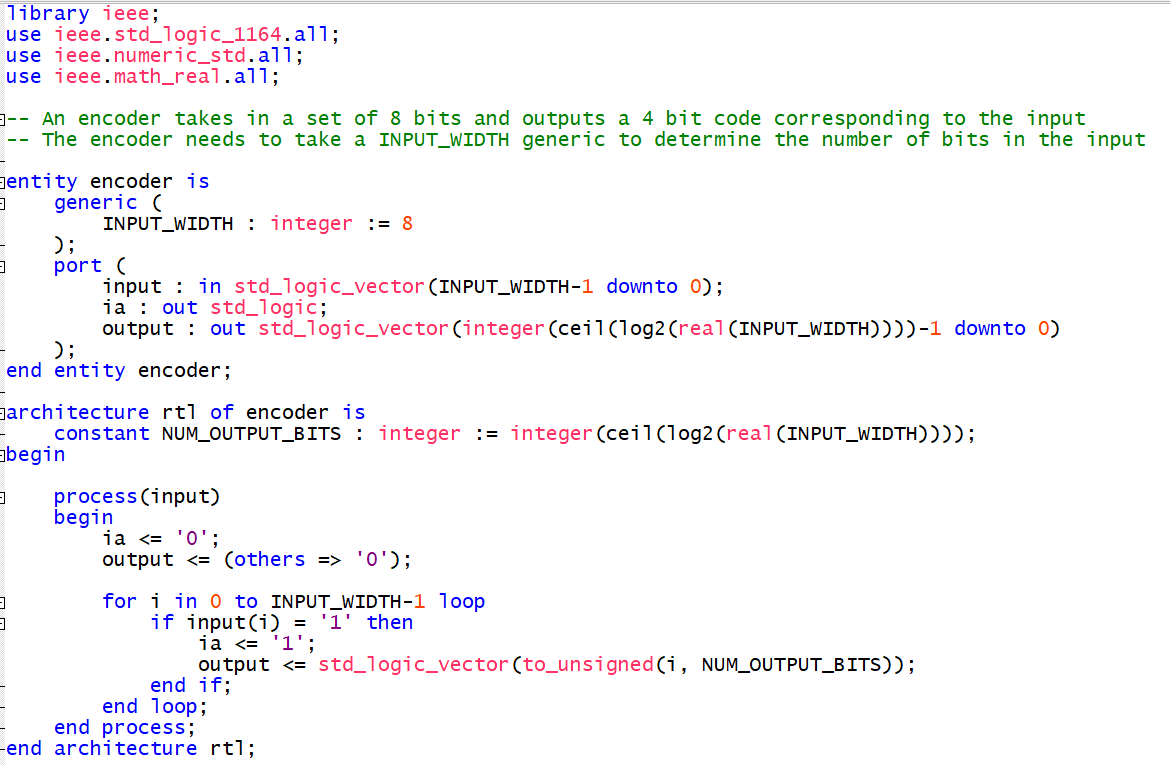
\includegraphics[scale=0.5]{Encoder_Impl.png}
    \caption{8-bit Encoder Implementation}
  \end{figure}

  % Simulation Results
  \begin{figure}[H]
    \centering
    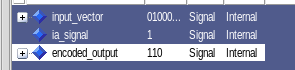
\includegraphics[scale=0.5]{encoder_tb.png}
    \caption{8-bit Encoder Simulation}
  \end{figure}
  \item 8-bit Decoder
  % Image of Implementation
  \begin{figure}[H]
    \centering
    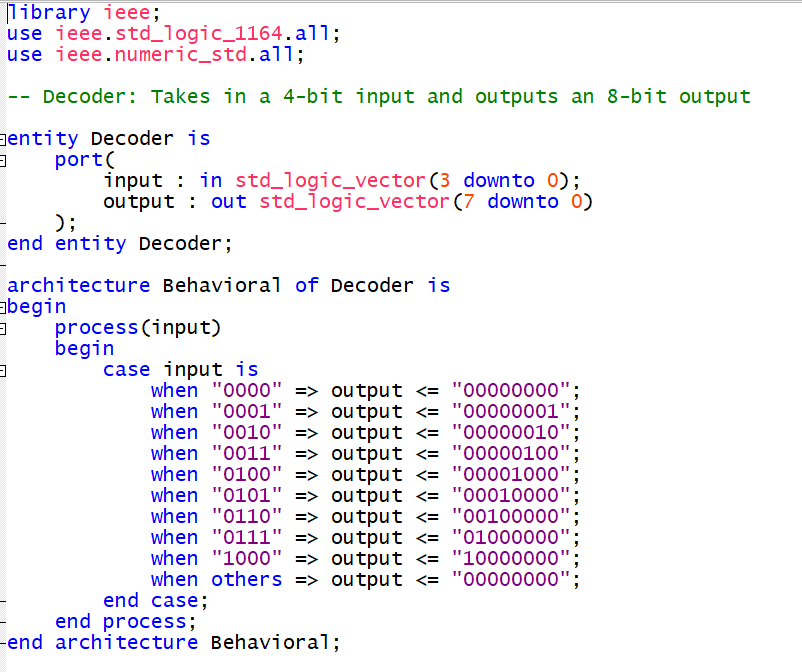
\includegraphics[scale=0.5]{Decoder_Impl.png}
    \caption{8-bit Decoder Implementation}
  \end{figure}

  % Simulation Results
  \begin{figure}[H]
    \centering
    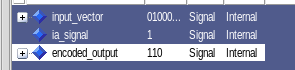
\includegraphics[scale=0.5]{encoder_tb.png}
    \caption{8-bit Decoder Simulation}
  \end{figure}
  \item 8-bit Multiplexer
  % Image of Implementation
  \begin{figure}[H]
    \centering
    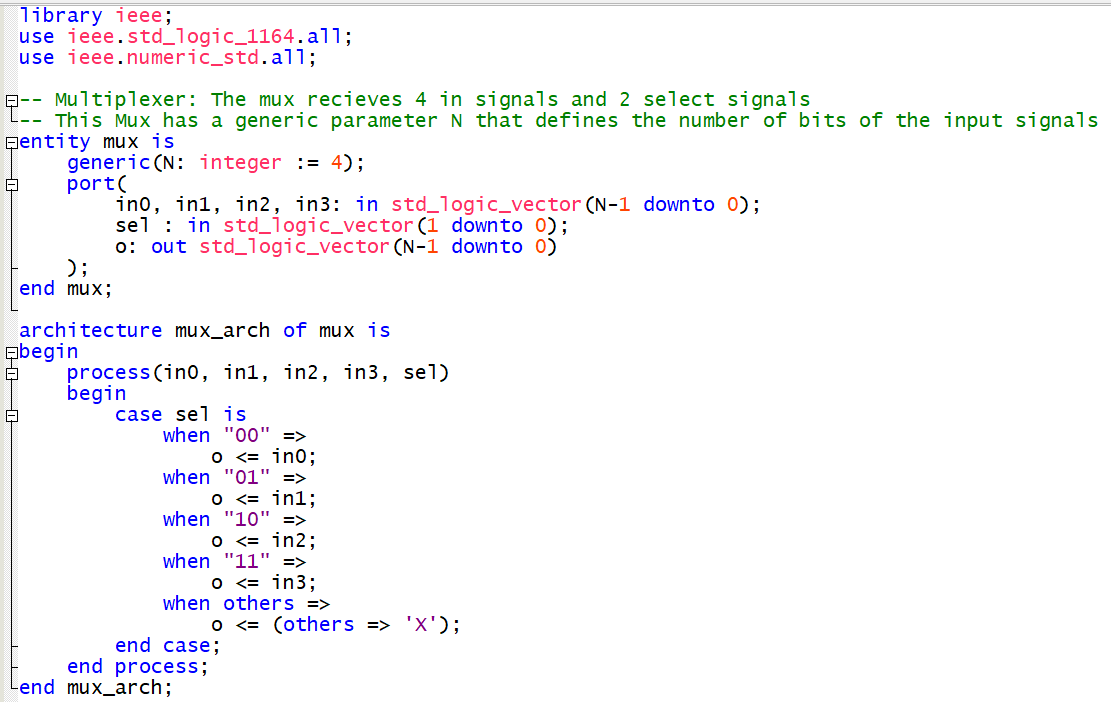
\includegraphics[scale=0.5]{mux_impl.png}
    \caption{8-bit Multiplexer Implementation}
  \end{figure}

  % Simulation Results
  \begin{figure}[H]
    \centering
    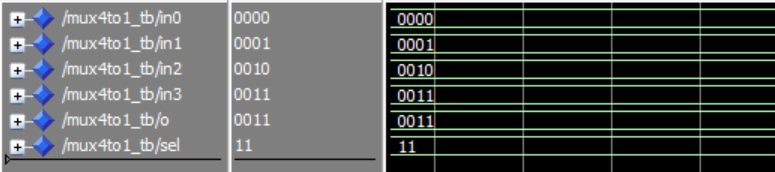
\includegraphics[scale=0.5]{mux_tb.png}
    \caption{8-bit Multiplexer Simulation}
  \end{figure}
  
  \item 8-bit Demultiplexer

  % Image of Implementation
  \begin{figure}[H]
    \centering
    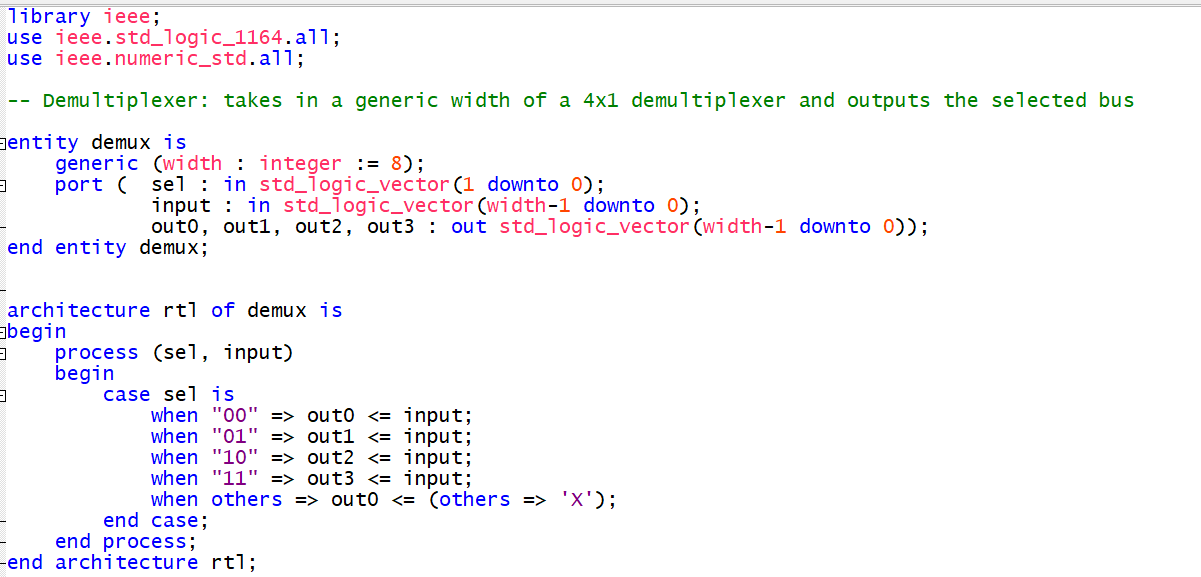
\includegraphics[scale=0.5]{demux_impl.png}
    \caption{8-bit Demultiplexer Implementation}
  \end{figure}

  % Simulation Results
  \begin{figure}[H]
    \centering
    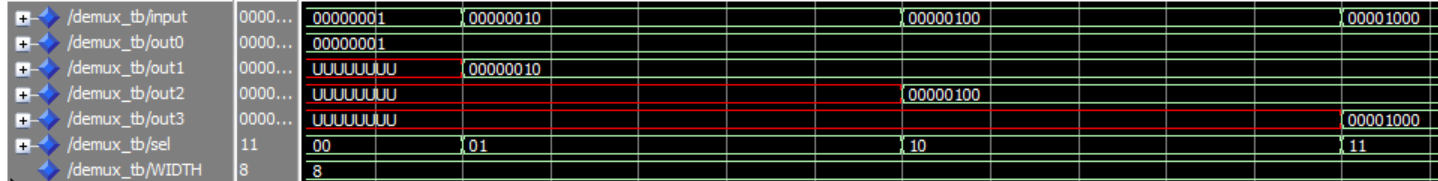
\includegraphics[scale=0.5]{demux_tb.png}
    \caption{8-bit Demultiplexer Simulation}
  \end{figure}
  \item Register

  % Image of Implementation
  \begin{figure}[H]
    \centering
    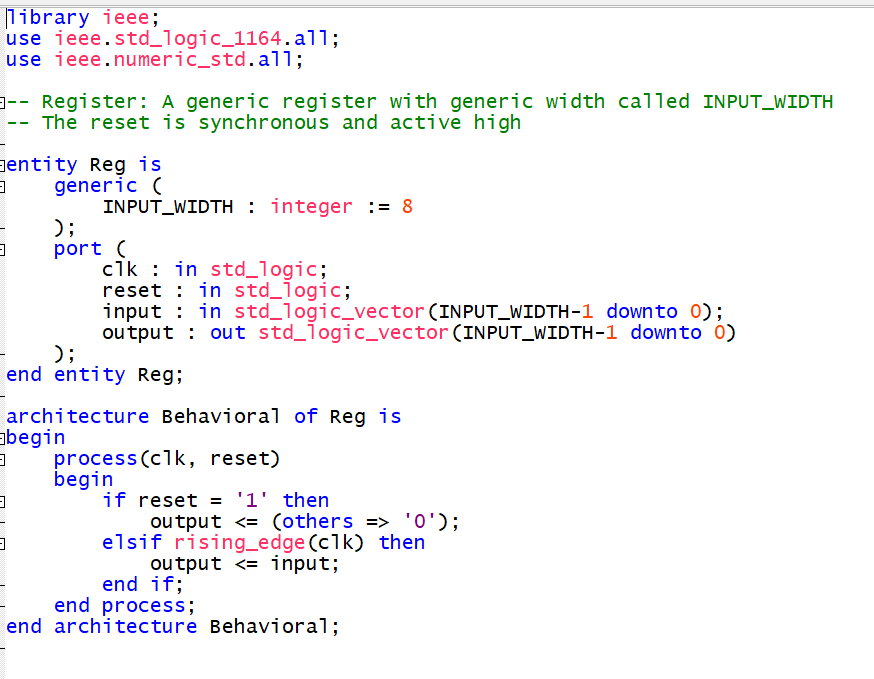
\includegraphics[scale=0.5]{reg_impl.png}
    \caption{Register Implementation}
  \end{figure}

  % Simulation Results
  \begin{figure}[H]
    \centering
    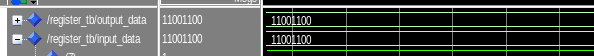
\includegraphics[scale=0.5]{reg_tb.png}
    \caption{Register Simulation}
  \end{figure}
\end{enumerate}

\subsubsection*{Part 2: Ripple Carry Adder}
\begin{enumerate}
  \item Implementation of RC Adder
  \begin{figure}[H]
    \centering
    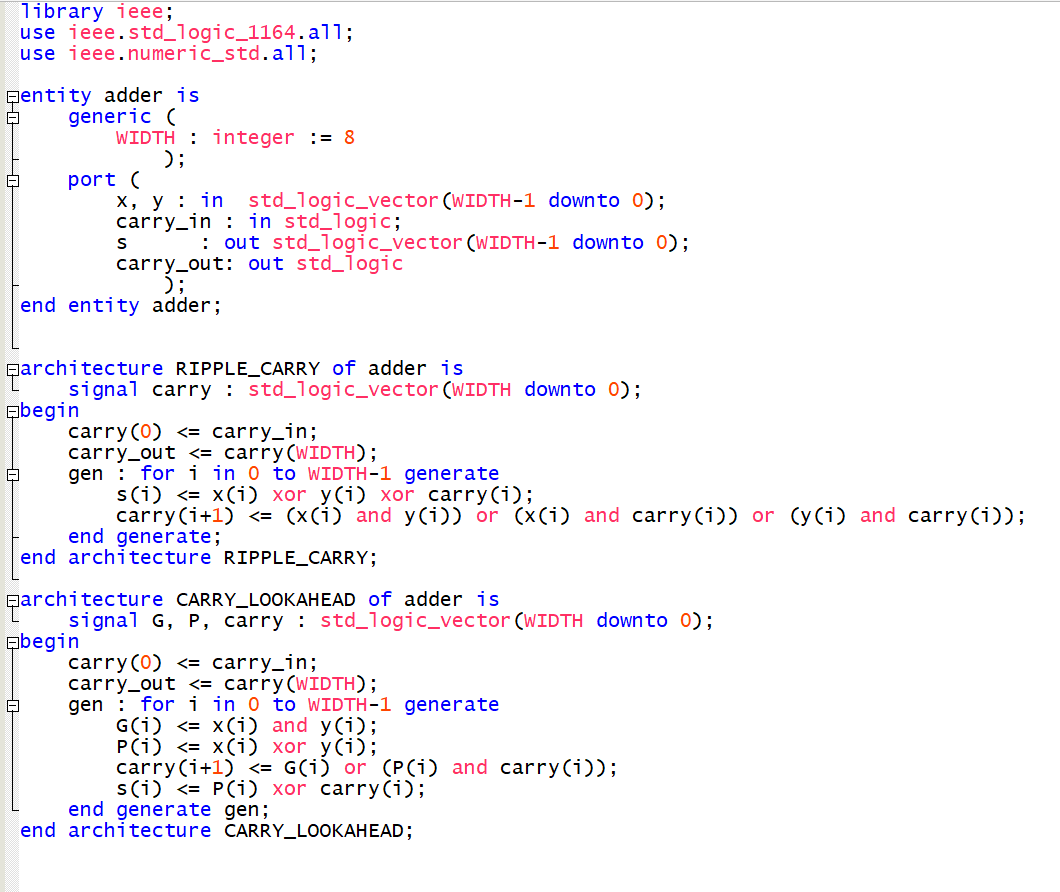
\includegraphics[scale=0.5]{adder_impl.png}
    \caption{Ripple Carry Adder Implementation}
  \end{figure}
\end{enumerate}

\subsubsection*{Part 3: Carry Lookahead Adder}
\begin{enumerate}
  \item Implementation of CL Adder
  \begin{figure}[H]
    \centering
    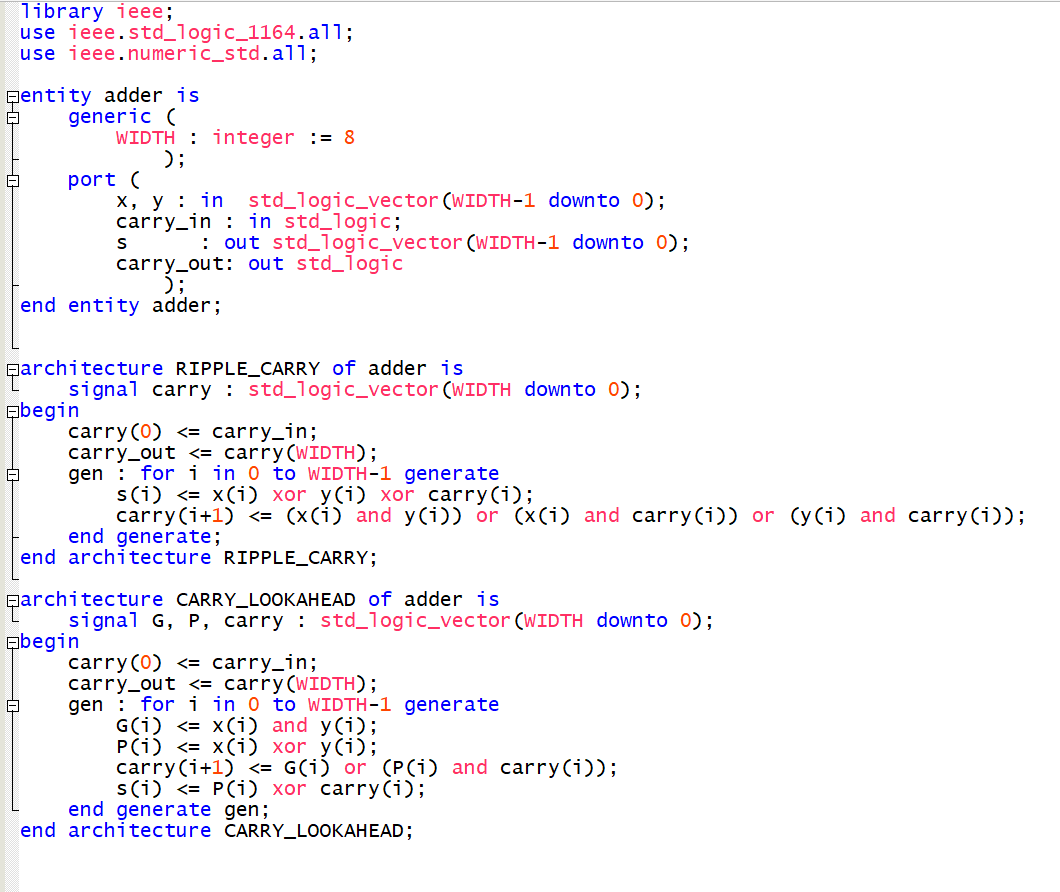
\includegraphics[scale=0.5]{adder_impl.png}
    \caption{Carry Lookahead Adder Implementation} 
  \end{figure}
\end{enumerate}

\subsection*{Reflection}
% Reflect on the learning and challenges faced during the prelab
I struggled to use the Questa Sim simulator and ended up deciding to use ModelSim instead. After I made the switch, I was able to complete the prelab without any issues. I learned a lot about the different components and how they can be used to build more complex systems. I also learned about the different types of signals and how they can be used to control the flow of data in a system.

\subsection*{Prelab Homework}
% Show all work for the Prelab Homework here

\section*{Postlab Report}

\subsection*{Problem Statement}
% Provide a short description of the lab’s goals, system, inputs, outputs, and function
% Section should be 1-2 paragraphs
The goal of Lab 1 focused on the design and implementation of various digital components. The lab required the design and simulation of an 8-bit encoder, 8-bit decoder, 8-bit multiplexer, 8-bit demultiplexer, and an 8-bit register. The lab also required the design and simulation of a ripple carry adder and a carry lookahead adder. The lab was designed to help students understand the basics of digital design and how to use various components to build more complex systems.

\subsection*{Design}
% Describe the design decisions, components, signals, and algorithms used
The overall design of the RTL components was relatively straightforward. The 8-bit encoder and decoder were designed using a case statement to map the input to the output. The multiplexer and demultiplexer were designed using a case statement to select the input or output based on the control signal. The register was designed using a process statement to control the flow of data. 

The ripple carry adder was more challenging than the previous components designed. The adder was designed to first allow for a generic input size. The logic used a for generate statement to create the full adders and connect them together. The carry lookahead adder was designed using a generate statement to create the carry lookahead logic and then connect the full adders together. The individual logic differed with in each for generate statement, but the overall structure was the same. The pros of using this design method allows for the components to be easily reused and modified.
\subsection*{Implementation}
% Describe the implementation process, time required, and any relevant code or pictures
As described before the implementation followed a similar pattern for each component. The 8-bit encoder and decoder were designed using a case statement to map the input to the output. The multiplexer and demultiplexer were designed using a case statement to select the input or output based on the control signal. The register was designed using a process statement to control the flow of data. The figure below shows the implementation of the 8-bit encoder as a base example.

\begin{figure}[H]
  \centering
  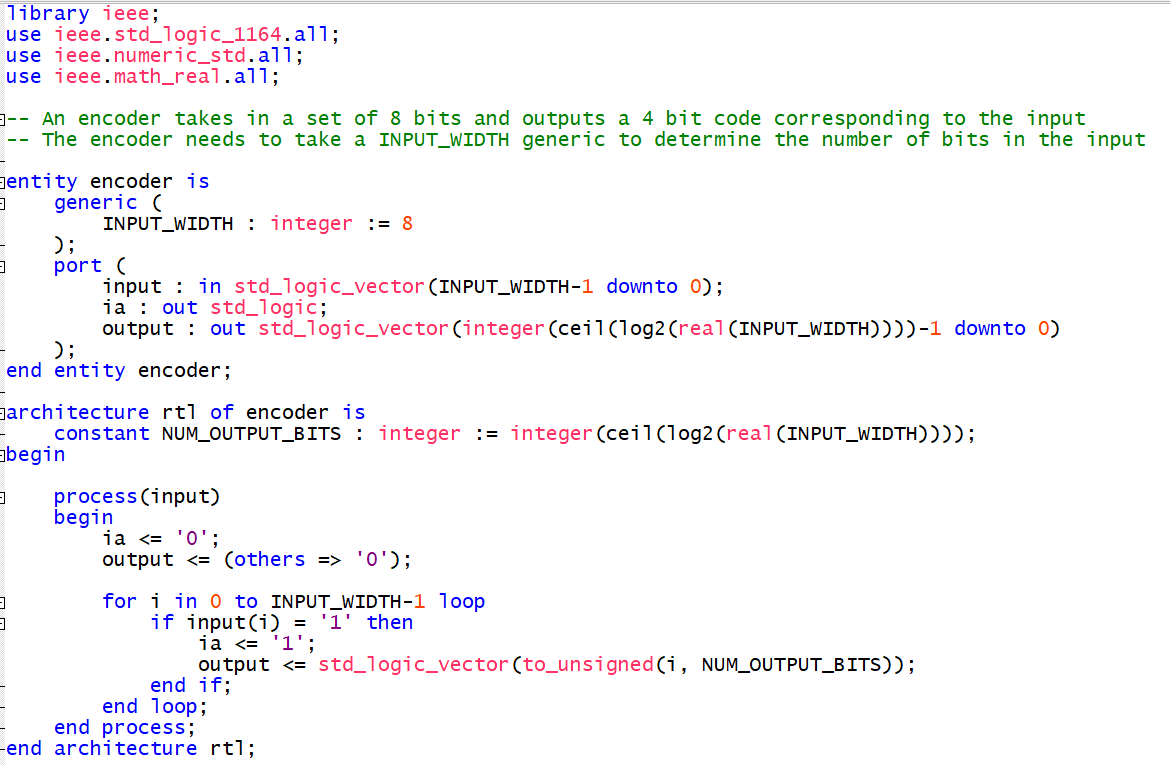
\includegraphics[scale=0.5]{Encoder_Impl.png}
  \caption{8-bit Encoder Implementation}
\end{figure}

The implementation of the ripple carry adder was more complex than the previous components. The adder was designed to first allow for a generic input size. The logic used a for generate statement to create the full adders and connect them together. The carry lookahead adder was designed using a generate statement to create the carry lookahead logic and then connect the full adders together. The individual logic differed with in each for generate statement, but the overall structure was the same. The figure below shows the implementation of the ripple carry adder and carry lookahead adder.

\begin{figure}[H]
  \centering
  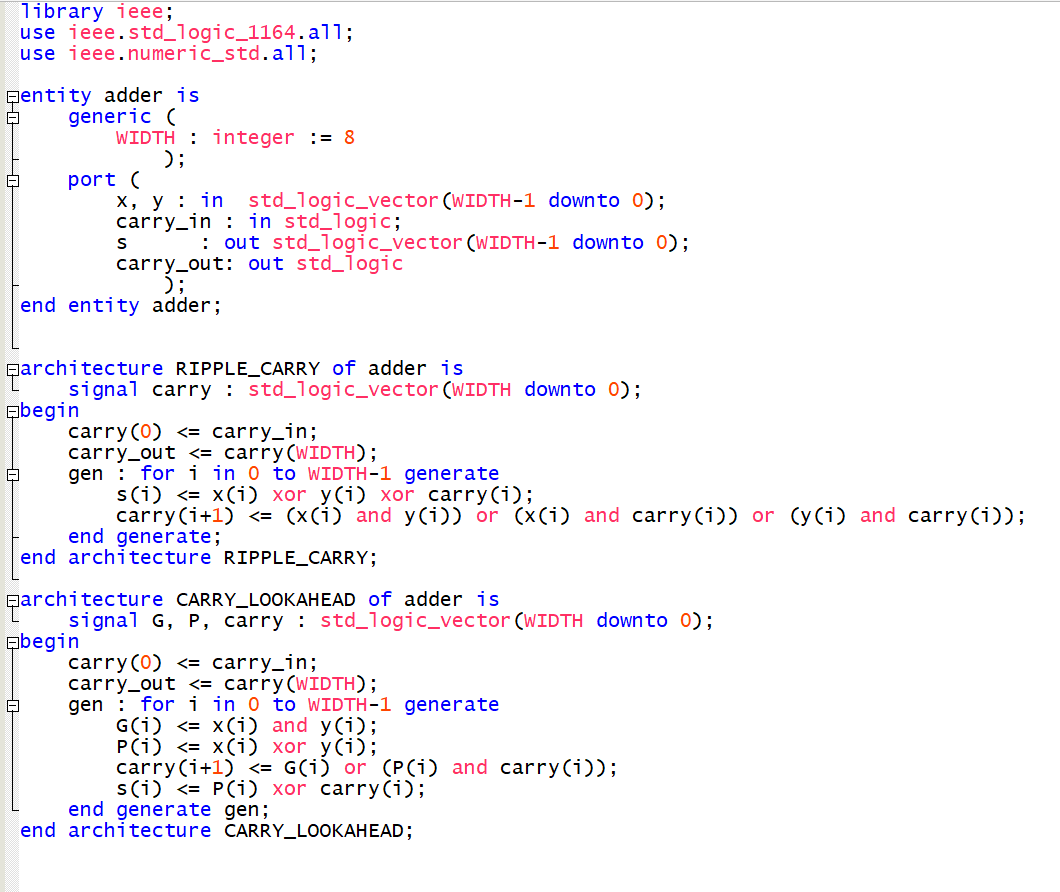
\includegraphics[scale=0.5]{adder_impl.png}
  \caption{Ripple Carry Adder Implementation}
\end{figure}
\subsection*{Testing}
% Explain how the design was tested and the outcomes

The design was tested using ModelSim. The testbench for each component was designed to test the functionality of the component. The testbench for the 8-bit demultiplexer is shown below.

\begin{figure}[H]
  \centering
  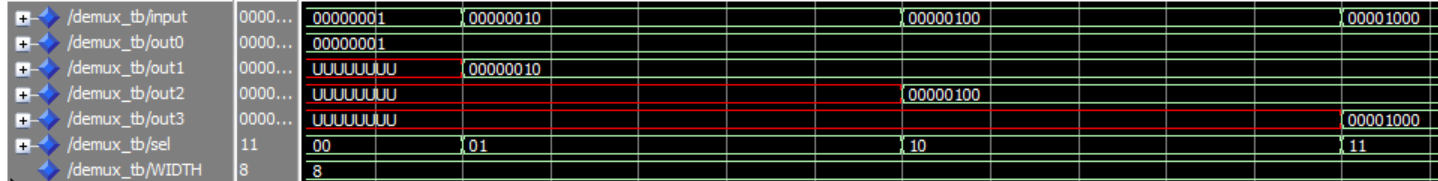
\includegraphics[scale=0.5]{demux_tb.png}
  \caption{8-bit Encoder Simulation} 
\end{figure}

The testbench for the ripple carry adder is shown below. It also includes the carry lookahead adder. The signals of the ripple carry adder are denoted with "rc" and the signals of the carry lookahead adder are denoted with "cl".

\begin{figure}[H]
  \centering
  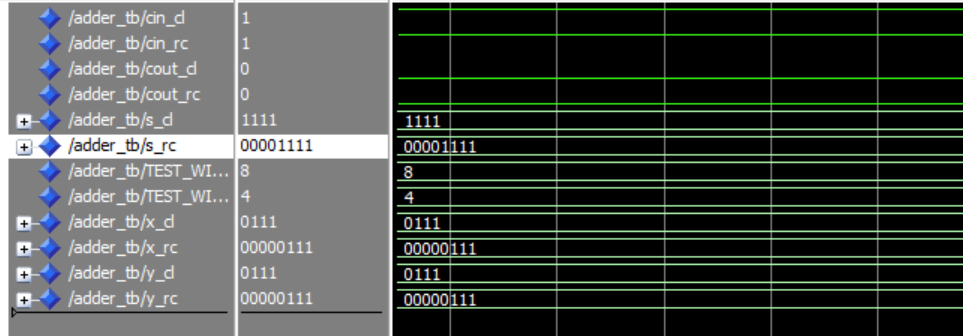
\includegraphics[scale=0.5]{adder_tb1.png}
  \caption{Adder Simulation}
\end{figure}

The second testbench for the adder is shown below. It is more simplistic.

\begin{figure}[H]
  \centering
  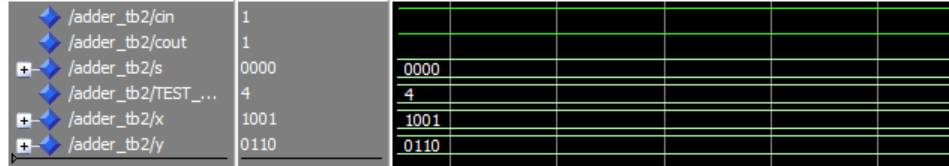
\includegraphics[scale=0.5]{adder_tb2.png}
  \caption{Adder Simulation 2}
\end{figure}

\subsection*{Conclusions}
% Summarize the work, successes, problems encountered, and future improvements
The work described in the report was more time intensive which reflects the learning process of the suite of tools at my disposal. The design and implementation of the components was relatively straightforward. The testing of the components was also straightforward. The only issue I encountered was using the Questa Sim simulator. I was able to resolve this issue by using ModelSim. The future improvements for the lab would be to use the Questa Sim simulator and to improve the testbenches for the components. Moving forward, challenges like the one I faced will be easier to overcome considering the tooling will remain the same for future labs.

\appendix
\section*{Appendix}
% Include all postlab code, screenshots, pictures, and simulations here
\end{document}
